\documentclass{beamer}
\usetheme{Dresden}
\usecolortheme{dove}
\setbeamertemplate{headline}{} % remove to add TOC back to top


% Packages
% ------------------
\usepackage{amssymb}
\usepackage{amsmath}
\usepackage{dsfont}
\usepackage{bm}
\usepackage{color}


% Commands
% ------------------
\newcommand{\sectionspace}{\vspace{3mm}}
\newcommand{\boxme}[1]{\fbox{\parbox{0.9\textwidth}{#1}}}
\newcommand{\fixme}{\textcolor{red}{\textbf{fix me}} \space}
\newcommand{\attention}[1]{\noindent \fixme \textcolor{red}{#1}}


% Header of Presentation
% ---------------------
\begin{document}
\title[{\makebox[.45\paperwidth]{\space\hfill%
    \insertframenumber/\inserttotalframenumber}}]{Correctness Guarantee for the
  Composition of Adaptive Cruise Control and Lane Keeping and Adaptive Cruise Control}
\subtitle{X. Xu, J.W. Grizle, P. Tabuada, and A.D. Ames}
\author[]{Presented by: Sergio Garc\'{i}a-Vergara}
\date{\today}

% title page
\frame{\titlepage}

% automatically generate table of contents
\frame{\frametitle{Table of Contents}\tableofcontents}



% @@@@@@@@@@@@@@@@@@@@@@@@@@@@@@@@@@@@@@@@@@@@@@@@@@


% comparison with Lyapunov functions
% -------------------------------------------
\section{What are Barrier Certificates?}
\frame{\frametitle{What are Barrier Certificates?}
\begin{itemize}

\item Also known as barrier functions, are used to verify temporal properties of
  a set without having to compute the system's reachable set.

\sectionspace
\item Recall \textbf{Lyapunov functions}: in control theory, these are linear
  functions used to prove the stability of a dynamical system.

\sectionspace
\item Let $\dot{x} = f(x)$ be the dynamics of a system with an equilibrium point
  at $x = 0$. The existence of a function $\bm{V(x) > 0 \: \forall x \neq 0}$
  such that $\bm{\dot{V}(x) \leq 0}$, guarantees the stability of the
  equilibrium point (asymptotical stability if $\dot{V}(x) < 0$).

\end{itemize}
}


% summary and definition of barier functions/certificates
% -------------------------------------------
\frame{\frametitle{What are Barrier Certificates?}
\begin{itemize}

\item Are used to design a family of control solutions that guarantee some nice
  properties about a set. Namely, \textbf{its forward invariance}.

\sectionspace
\item Given dynamics $\dot{x} = f(x)$ and a trajectory $x(t, x_o)$, set $S$ is
  called \textit{forward invariant} if:

\sectionspace
\boxme{\centering for every $x_o \in S$ implies that
  $\bm{x(t, x_o) \in S \; \forall t = 0}$.}

\sectionspace
\item Nice because we can define a \textit{safety set} and guarantee that our
  system will always meet its constraints.

\end{itemize}
}


% equations and more details on barrier certificates
% -------------------------------------------
\subsection{Definition: Barrier Certificates}
\frame{\frametitle{Definition: Barrier Certificates}
\begin{itemize}
\item Consider a system with dynamics $\dot{x} = f(x)$ and a closed set \\

  \begin{equation*}
    C = \{x \in \mathbb{R}^n \: | \: h(x) \geq 0\}
  \end{equation*}

  for some continuously differentiable function
  $h : \mathbb{R}^n \mapsto \mathbb{R}$.

\sectionspace
\item If there exists a constant $\gamma > 0$ and a set $D$ with
  $C \subseteq D \subset \mathbb{R}^n$ such that:

  \begin{equation*}\label{eq:barrier_function}
    \bm{\dot{h}(x) \geq -\gamma h(x), \; \forall x \in D}
  \end{equation*}

  then:

  \sectionspace
  \boxme{\centering the function $h(x)$ is called a \textbf{\textit{barrier
        function}}.}
\end{itemize}
}


% general theorem
% -------------------------------------------
\subsection{General Theorem}
\frame{\frametitle{General Theorem}
\begin{itemize}

\item Consider an affine control system: \\

\begin{equation*}
\dot{x} = f(x) + g(x)u
\end{equation*}

with $x \in \mathbb{R}^n$ and $u \in \mathbb{R}^m$.

\sectionspace
\item Given a set $C = \{x \in \mathbb{R}^n \: | \: h(x) \geq 0\}$ for a
  continuously differentiable function $h$. If $h$ is a control barrier function
  then any controller $\bm{u(x) \in K_{zcbf}(x)}$ will render the set $C$
  \textbf{forward invariant}.

\sectionspace
\boxme{\centering
  $K_{zcbf}(x) = \{u \in U \: | \: L_fh(x) + L_gh(x)u + \gamma h(x) \geq 0\}$}
\end{itemize}
}


% problem formulation
% -------------------------------------------
\section{Problem Formulation: Dynamics and Safety Constraints}
\frame{\frametitle{Problem Formulation}
\begin{itemize}

\item Control objectives:

\begin{itemize}
\item \textbf{LK}: Control the steering of an autonomous car to maintain lane
  centering.
\item \textbf{ACC}: maintain a safe following distance when a preceeding vehicle
  is driving at a lower speed.
\end{itemize}

\sectionspace
\item Safety constraints for LK and ACC are expressed in terms of set
  invariance.

\sectionspace
\item Controlled invariant sets are used to encode both the correct behavior of
  the closed-loop system and a set of feedback control laws that will achieve
  it.
\end{itemize}
}


% lane keeping dynamics
% -------------------------------------------
\subsection{Lane Keeping}
\frame{\frametitle{Lane Keeping: Dynamics}
\begin{itemize}

\item Lateral-yaw model: \\

\begin{equation*}
\begin{split}
\bm{\dot{x}}_1 & = f_1(\bm{x}_1, v_f) + g_1(\bm{x}_1)u_1 + \Delta f_1(d) \\
\bm{x}_1 & := (y, v, \Delta\Psi, r)'
\end{split}
\end{equation*}

\begin{itemize}
\item $y$: lateral displacement from the center of the lane
\item $v$: lateral velocity
\item $\Delta\Psi$: yaw angle deviation in road-fixed coordinates
\item $r$: yaw rate

\sectionspace
\item $u_1 = \delta_f$: steering angle of the front wheels
\item $d$: desired yaw rate (computed from road curvature)
\end{itemize}

\end{itemize}
}


% lane keeping safety constraints
% -------------------------------------------
\frame{\frametitle{Lane Keeping: Safety Constraints}
\begin{itemize}

\item Main constraint: Keep the car within its lane (i.e. constrain the lateral
  displacement):
\begin{center} $|y| \leq y_m$ \end{center}

\sectionspace
\item Set of hard constraints for LK:

\sectionspace
\boxme{
\begin{equation*}
\begin{split}
\mathcal{X}_{LK} := & \{\bm{x}_1 \in \mathbb{R}^4 \: | \\
& |y| \leq y_m, |v| \leq v_m, |\Delta \Psi| \leq \Delta \Psi_m, |r| \leq r_m\}
\end{split}
\end{equation*}
}

\sectionspace
\item Optional soft constraint: set an upper bound for the lateral acceleration
  to respect the driver's comfort.

\end{itemize}
}


% adaptive cruise control dynamics
% -------------------------------------------
\subsection{Adaptive Cruise Control}
\frame{\frametitle{Adaptive Cruise Control: Dynamics}
\begin{itemize}

\item Point-mass model: \\

\begin{equation*}
\begin{split}
\bm{\dot{x}}_2 & = f_2(\bm{x}_2) + g_2(\bm{x}_2)u_2 + \Delta f_2(vr, a_L) \\
\bm{x}_2 & := (v_f, v_l, D)'
\end{split}
\end{equation*}

\begin{itemize}
\item $v_f$: following car's speed
\item $v_l$: lead car's speed
\item $D$: distance between the two cars

\sectionspace
\item $u_2 = F_w$: longitudinal force developed by the wheels
\item $F_r$: aerodynamic drag
\item $a_L$: overall acceleration/deceleration of the lead car
\end{itemize}

\end{itemize}
}


% adaptive cruise control safety constraints
% -------------------------------------------
\frame{\frametitle{Adaptive Cruise Control: Safety Constraints}
\begin{itemize}

\item Main constraint: the controlled vehicle should maintain a safe distance
  from the lead car. Paper uses this formulation:

\sectionspace
\boxme{
\begin{equation*}
D \geq \tau_d v_f + D_o
\end{equation*}
}

\sectionspace
where $\tau_d$ is the desired time headway and $D_o$ is the minimal distance
between cars when they are fully stopped.

\sectionspace
\item Soft constraint: achieve a desired speed $v_d$ set by the driver:

\begin{equation*}
\lim_{t \to \infty} v_f(t) - v_d = 0
\end{equation*}

\end{itemize}
}


% methodology
% -------------------------------------------
\section{Methodology}
\frame{\frametitle{Methodology}
\begin{itemize}
\item \textbf{GOAL:} Barrier certificates seek a function whose sub-level sets
  are all invariant, without the difficult task of computing the system's
  reachable set.
\end{itemize}

\begin{enumerate}
\item Construct a controlled invariant set that encodes the safety
  specifications.
\item Construct a feedback law that ensures that trajectories of the controlled
  system are confined within the set.
\end{enumerate}
}


% results
% -------------------------------------------
\section{Simulation Results}
\frame{\frametitle{Simulation Results}
\begin{figure}[h]
\begin{center}
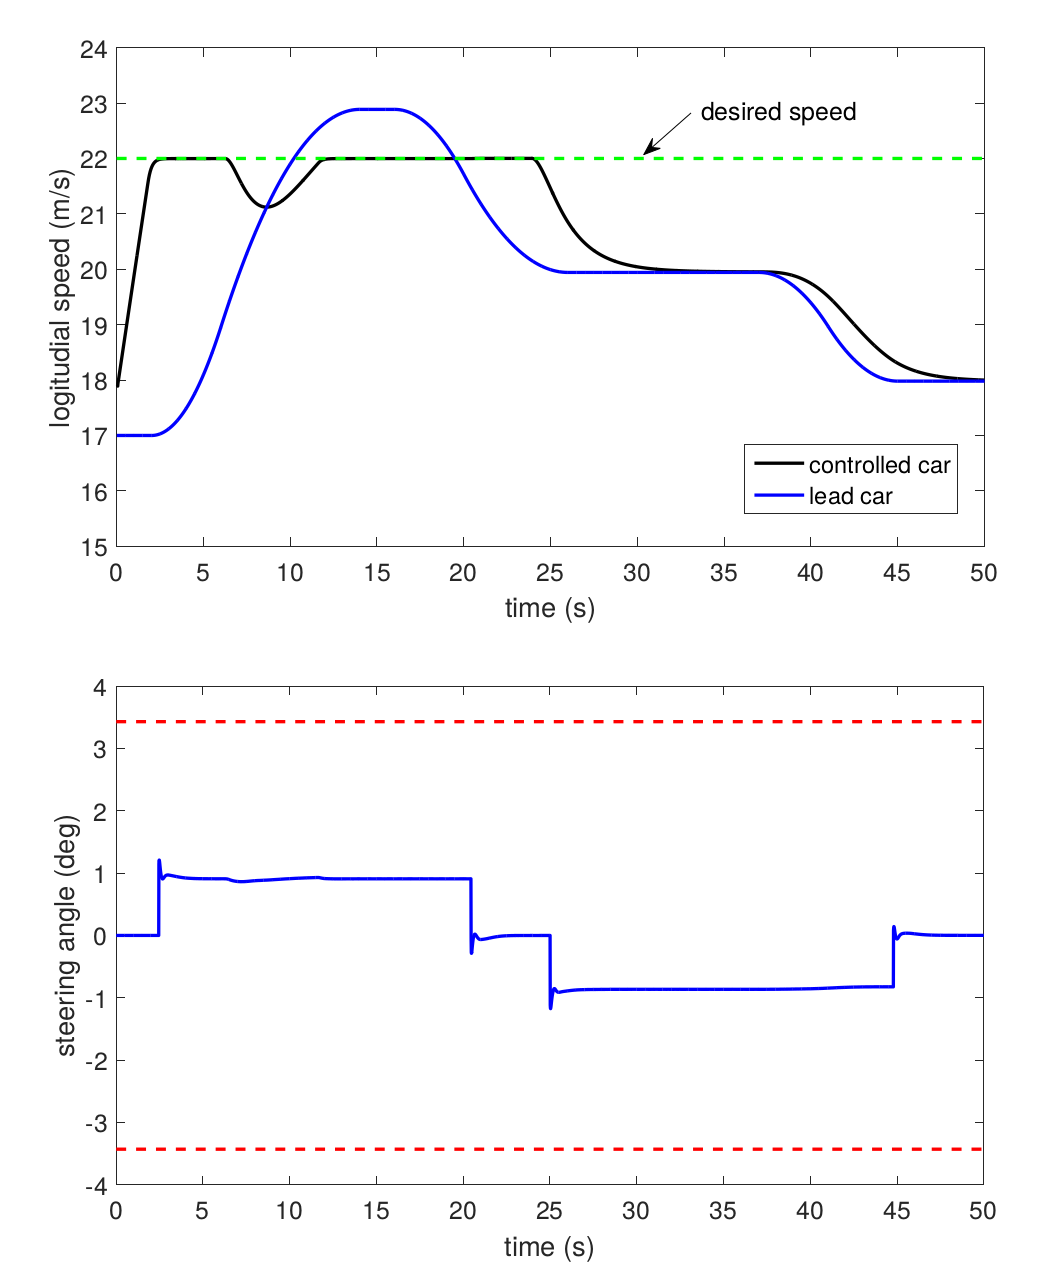
\includegraphics[scale=0.17]{figs/simulation_results.png}
\end{center}
 % \caption{The safe set $C$ is the shaded region.}
\label{fig:simulation_results}
\end{figure}
}


% conclusions
% -------------------------------------------
\section{Conclusions}
\frame{\frametitle{Conclusions}
\begin{itemize}

\item Longitudinal force and steering angle are generated by solving quadratic
  programs.

\sectionspace
\item The safety constraints are hard constraints that are enforced by confining
  the states of the vehicle within determined controlled-invariant sets.
\begin{itemize}
\item The performance objectives are soft constraints that can be overridden
  when they are in conflict with safety.
\end{itemize}

\sectionspace
\item Any control laws respecting the contracts given for LK and ADD will
  guarantee safety of the closed-loop system when the two modules are activated
  simultaneously.
\end{itemize}
}


% Thank You
% -------------------------------------------
\frame{\frametitle{Questions?}
\centering Thank You!
}


% ==========================================
% backup slides
% ==========================================



% barrier certificates example
% -------------------------------------------
\frame{\frametitle{Example: Barrier Certificates}
\begin{figure}[h]
\begin{center}
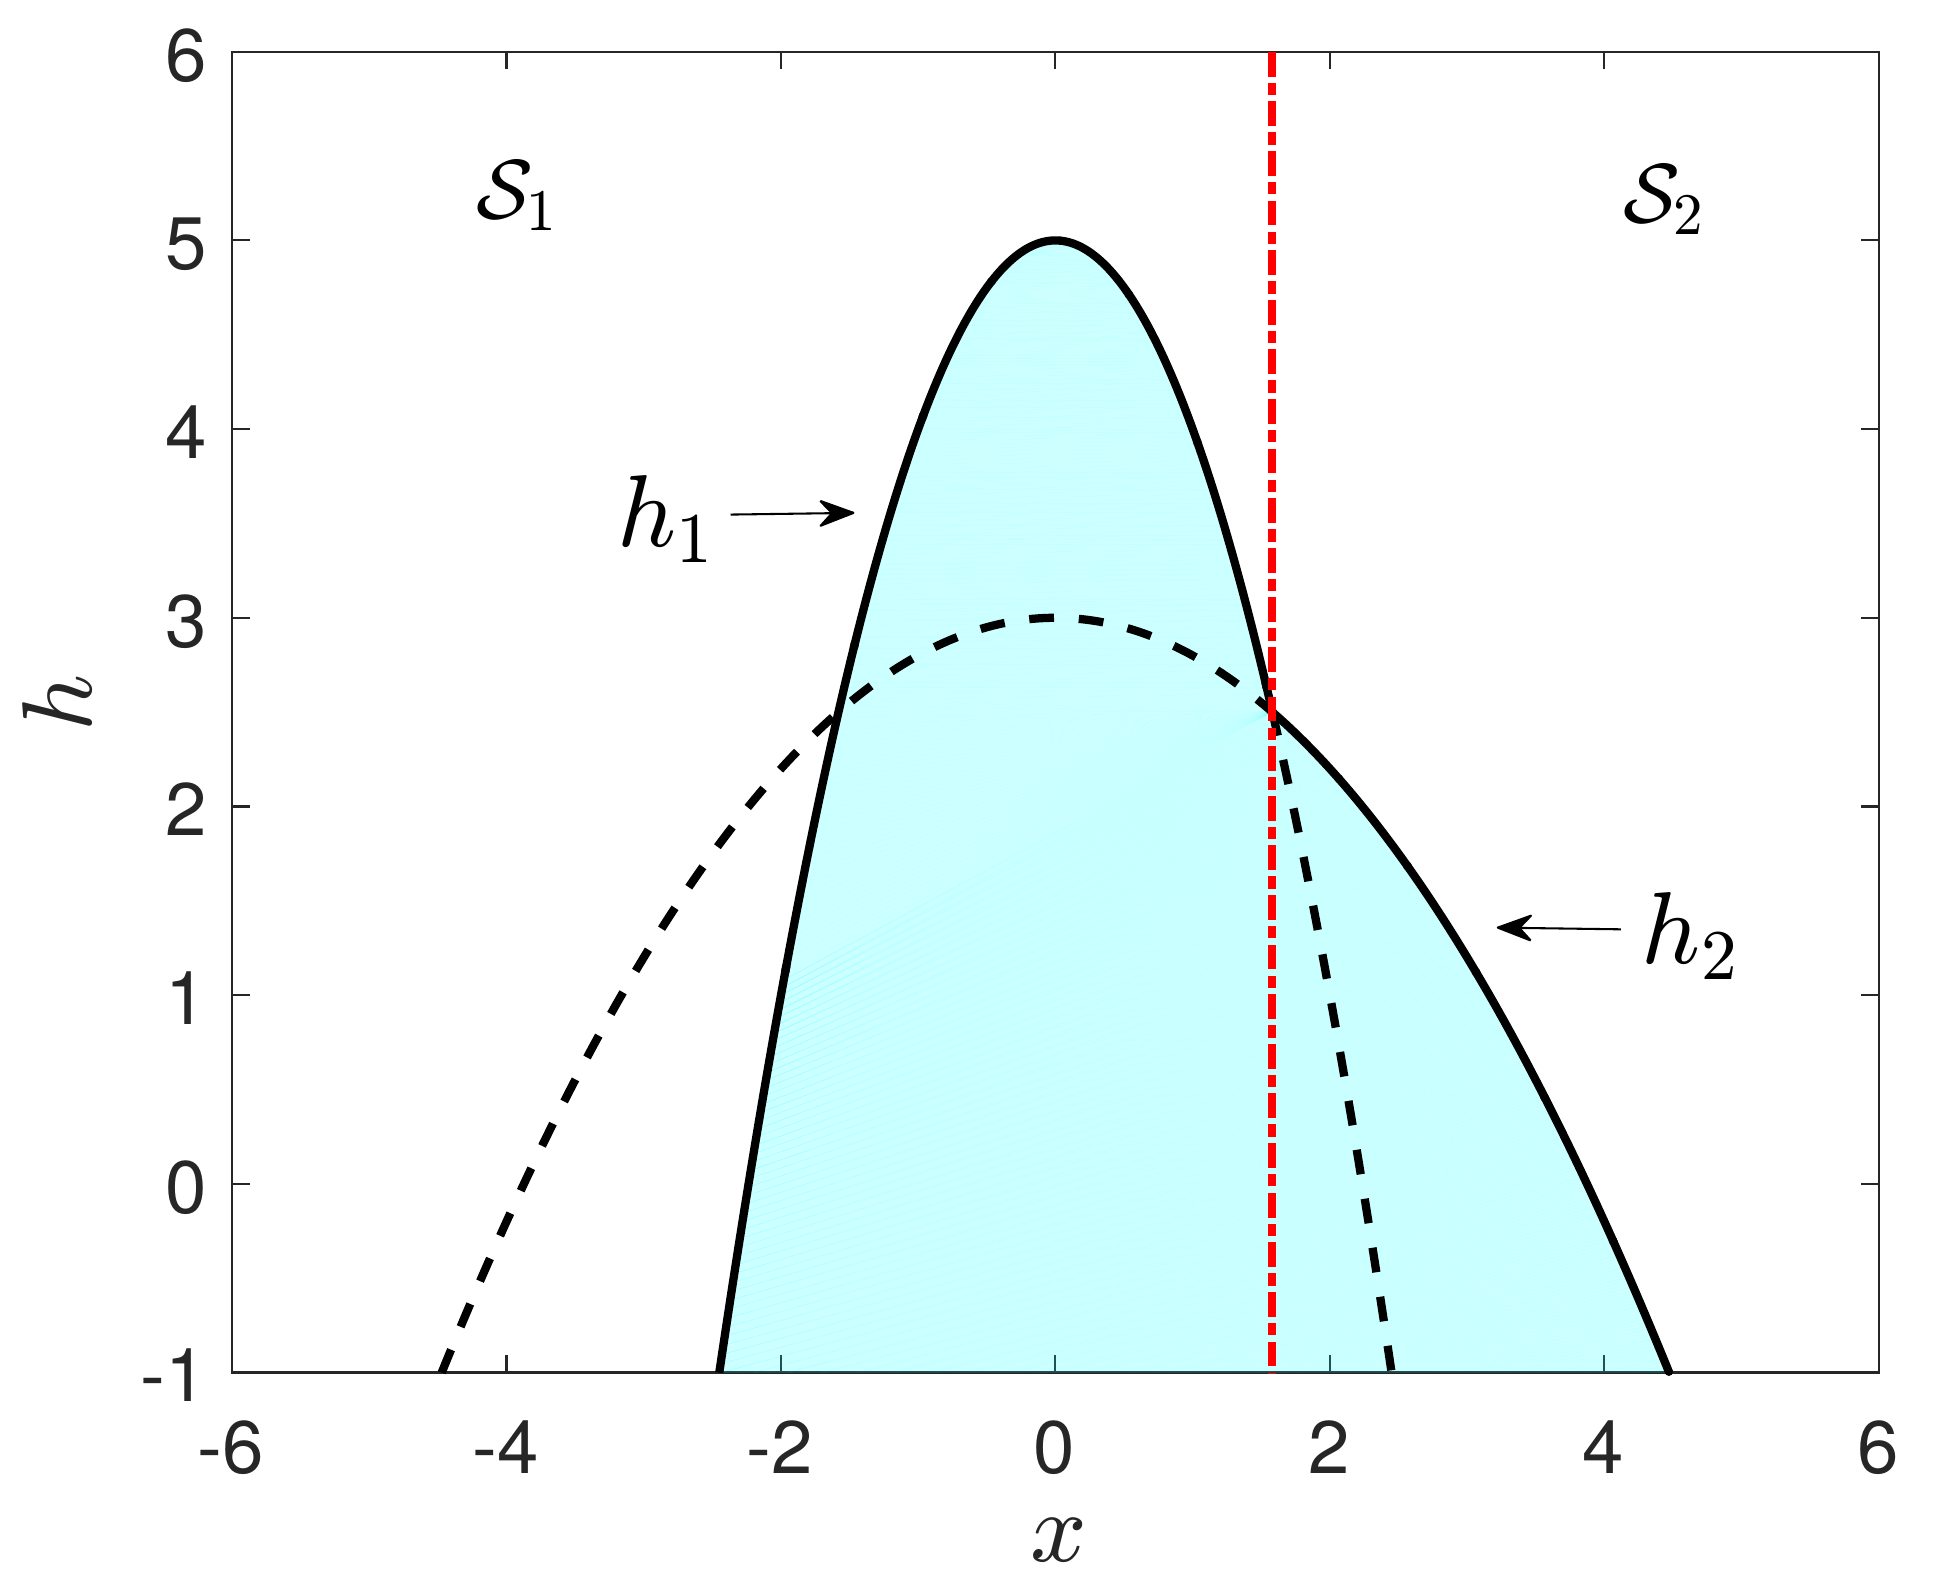
\includegraphics[scale=0.09]{figs/barrier_certificates_example.png}
\end{center}
 % \caption{The safe set $C$ is the shaded region.}
\label{fig:barrier_certificates_example}
\end{figure}

\begin{itemize}
\item Functions: $h_1(x) = -x^2 + 5$ and $h_2(x) = -0.2x^2 + 3$
\item Partitions: $S_1 = (-\infty, \sqrt{10}/2]$ and $S_2 = [\sqrt{10}/2,
  \infty)$

\sectionspace
\boxme{\centering Safe set: $C := \{x | h(x) \geq 0\}$ is the shaded area.}
\end{itemize}
}


% algorithm: syntesis of control barrier functions for LK
% -------------------------------------------
\frame{\frametitle{Example: Barrier Certificates}
\begin{figure}[h]
\begin{center}
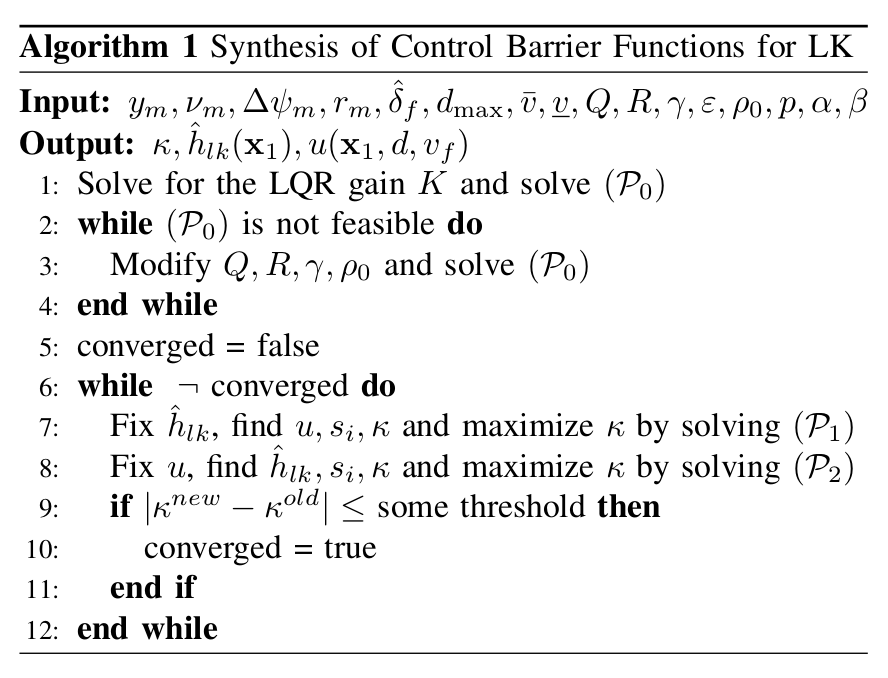
\includegraphics[scale=0.26]{figs/algorithm_CBF_LK.png}
\end{center}
 \caption{Algorithm for the Synthesis of Control Barrier Functions for LK.}
\label{fig:algorithm_CBF_LK}
\end{figure}
}


% -------------------------------------------
\end{document}


%%% Local Variables:
%%% mode: latex
%%% TeX-master: t
%%% End:
